\section{PCA}
%Plot examples of good and bad projections after PCA. Discuss in what these are good or bad projections. Discuss the eigenvalues of these projections.

	The goal of PCA is to project our dataset into a new compact base which keeps enough variance of data (i.e. information). Processing high-dimensional data requires lot of computational resources. Thus, we need to reduce the dimension of data using PCA in order to extract the main features. Firstly, we load the dataset 1 into \texttt{MLDEMOS} and split the two different classes. On figure \ref{fig:figure2}, we show the eigen value of each component projected and the reconstruction error function of eigen vectors. We decided to keep approximately 80\% of variance, therefore the 12 first eigen vector are used to compute the PCA.  \\
\begin{figure}[ht]
\centering
    \centering
	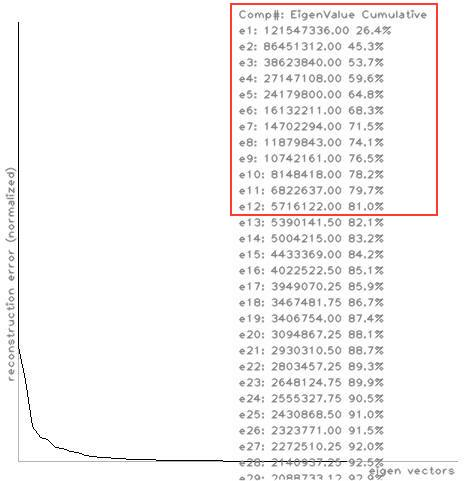
\includegraphics[height=0.1\textheight]{pca/Eigenvalue.jpeg}
	\caption{Eigen value cumulative and reconstruction error}
	\label{fig:figure2}
\end{figure}
	After applying the PCA on our dataset, we obtain several eigenvectors, we will introduce two of them with a manual graphical classification. Firstly, the primary eigenvectors, figure \ref{fig:figure3_1}, shows a well separation between the two classes with no overlapping between samples. Contrary to the first scatterplot, the separation of the classes in the second one, figure \ref{fig:figure3_2}, is not very accurate. We can observe an overlap; some of the data points in class 1 are inside the cluster of class 2, thus, this scatterplot doesn't represent efficiently our classes for a classification step.  
%Discuss the eigenvalues of these projections.
The eigenvalue of the primary plan is 45,3 \% comparing to 34,8 \% for the second one. That means the primary plan contains more information than the second one.   
Therefore, we decide to choose the primary projection to perform the classification.
\begin{figure}[!ht]
\centering
	\begin{subfigure}[h]{0.47\textwidth}
    \centering
	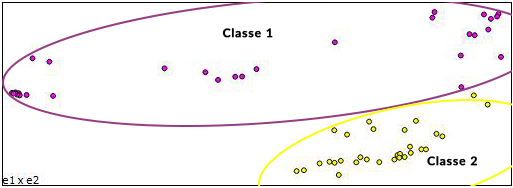
\includegraphics[width=0.8\textwidth,height=0.08\textheight]{pca/Scatter1.jpg}
	\caption{\bf Scatterplot with eigenvector 1 x 2}
	\label{fig:figure3_1}
	\end{subfigure}
    \begin{subfigure}[h]{0.47\textwidth}
    \centering
  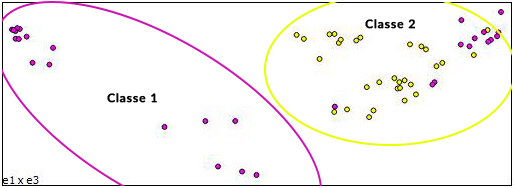
\includegraphics[width=0.8\textwidth,height=0.08\textheight]{pca/Scatter2.jpg}
	\caption{\bf Scatterplot with eigenvector 1 x 3}
	\label{fig:figure3_2}
    \end{subfigure}
\caption{Separation of the classes with PCA}
\end{figure}